\documentclass{sig-alternate-05-2015}
\usepackage{hyperref}


\begin{document}

% Copyright
%\setcopyright{acmcopyright}
% DOI
\doi{insert doi here}

% ISBN
\isbn{insert isbn here}

\title{BigBInf Micro Cloud Platform}

\numberofauthors{1}
\author{
% 1st. author
\alignauthor
Brendan D. Ball\\
       \affaddr{University of Cape Town}\\
}

\date{30 August 2015}


\maketitle
\begin{abstract}
[Abstract]
\end{abstract}
\keywords{Big Data; BioInformatics; Clouds}


\section{Introduction}
Cloud infrastructure is the combination of multiple compute and storage resources presented as a single system on the internet. Cloud computing has developed considerably over the last decade. Examples of commercial cloud offerings include Amazon Web Services and Google Compute Engine \cite{krishnan2015google, mathew2014overview}. Cloud infrastructure has the potential to simplify the processing of big data sets, as well as collaboration between remote researchers. 
\\
\\
The first step in simplifying processing of big data sets is to minimize the need for transferring the data. This can be done by storing the data in a cloud and allow researchers access to process the data on the cloud instead of downloading the data first before processing it. Minimizing the need for transferring Big Data is important because limitations in current internet infrastructure makes collaboration difficult when Big Data is involved. 
\\
\\
When using a commercial cloud such as Amazon EC2, the problem of uploading big data sets to their cloud infrastructure still exists \cite{baker2010next}. Micro clouds deployed on-site would overcome this challenge by keeping the data locally, while still reaping the benefits of a cloud platform. However, with different research institutions deploying their own micro clouds, cloud interoperability is required to allow researchers from different institutions to collaborate on the same data. The cloud interoperability creates a community cloud. A use-case of a specific community cloud  by Jimenez et al. \cite{jimenez2014deploying} contains core architectural properties needed for a successful community cloud. These properties include autonomy (where each micro cloud is be managed independently), security, self management of nodes, and scalability.
\\
\\
The traditional approach to creating a cloud platform allows users to run their own instances of operating systems (such as Amazon EC2) via virtualisation technology. This includes both hardware level emulation support and the software needed to manage the virtualisation. These virtualisation schemes use machine level virtualisation \cite{fink2014docker}. \\\\
A new method, known as containerization, provides much of the same functionality, with added benefits of lower resource usage and better performance. Containers are able to run native machine instructions compared to virtualisation emulating every machine instruction \cite{dua2014virtualization}. Containers are only useful when complete virtualisation is not needed, but allow for isolated application deployment and portability. Using containers instead of virtual machines has only recently become popular. The growth in popularity has resulted in a number of systems being developed including Rancher and Kubernetes. 
\\\\
Both virtualisation and containerization requires every instance to be configured by installing required software packages. Configuration can be time consuming, particularly in the context of bioinformatics. Cloud BioLinux is part of a cloud solution which solves this issue \cite{krampis2012cloud}. This toolkit makes it easy to deploy virtual machines to a cloud platform with bioinformatics infrastructure pre-configured. It bundles specific packages used in next generation sequence analysis (which is the processing of DNA data), thereby decreasing configuration time and increasing maintainability. Instances of Cloud BioLinux have been tested on the Amazon EC2 cloud platform and on a private Eucalyptus cloud. Eucalyptus is open source cloud software that enables you to create your own private cloud.
\\\\
Another project compatible with both Amazon EC2 and Eucalyptus is CloudMan \cite{afgan2015building}. CloudMan is designed as a workbench which manages cloud resources. A workbench relies on a pre-configured environment on which to execute code. It is aimed at improving biomedical data anaylsis and fully integrates with the Galaxy framework, a biomedical research platform. This cloud solution does not provide a user configurable execution environment as it relies on Galaxy tools to perform analyses. 
\\\\
We aim to provide users with a configurable environment by taking advantage of open source cloud software and Linux containers to enable efficient processing of Big Data through the use of micro clouds. The aim is to build a micro cloud platform and form a community cloud which allows sharing of data and collaboration of users between multiple micro clouds. Users can access data and submit jobs to the micro cloud by interacting with a front end web interface. Evaluation is done by deploying two micro clouds, one at UWC and one at UCT. The functionality is evaluated by uploading sample code and executing it on data which already exists on the cloud.
\\\\
UCT and UWC are collaborators on this project. UWC provided valuable hardware resources enabling thorough evaluation in a real world setting.

\section{Background}
Docker is built on top of Linux containers and is the main technology that we are using to build the micro cloud. To build a micro cloud platform a cluster manager is required. We look at OpenStack and Kubernetes as possible systems for a cluster manager.


\subsection{Docker}
Docker is an implementation of a Linux container management tool. Docker functions similarly to virtualisation. It uses an image to quickly launch a pre-configured isolated environment. The key difference is that containers directly uses the Linux kernel on the host machine to run native instructions. Containers are lightweight and launched in a fraction of time of a virtual machine \cite{joy2015performance}. 
\\\\
Docker builds on Linux containers by implementing an image format which makes use of an AUFS filesystem. This allows a docker image to be built up from a number of intermediate layers. Layers can be added or removed without affecting another layer in the image \cite{boettiger2014introduction}.
\\\\
The layered approach to creating a Docker image allows images to be built using a script called a Dockerfile. Defining an image with a script makes docker images much more portable and reproducible compared to creating an image from a running environment, as is the case with virtualisation \cite{boettiger2014introduction}.

The Docker group also hosts a publicly available image repository where anyone can upload or download available Docker images. These images provide full disclosure of its configuration via its Dockerfile. This provides great community support as you will often find that an image already exists for specific use-cases. An example is of CloudBioLinux which officially only provides virtual machine images, however third parties have uploaded Docker images of CloudBioLinux available for anyone to use.

\subsection{OpenStack}
Openstack is a full stack cloud platform which manages compute, storage, and networking resources. OpenStack can be used to orchestrate virtual machines and has recently been extended to support docker containers as well. OpenStack aims to be a complete cloud solution which has resulted in it being cluttered, with many-inter dependent components \cite{affetti2015adock}. The required functionality  from a cluster manager for this project is limited compared to everything that OpenStack provides. A simpler cluster manager, specifically designed for use with docker is better suited for this project.


\subsection{Kubernetes}
Kubernetes is a pure container manager specifically designed to orchestrate docker containers. A new system, Kubernetes version 1 has recently been released. Kubernetes looks most promising as it is easy to use. Given that it is relatively new it is not cluttered and aims to solve a single problem of being a container manager \cite{googleborg}. 
\\\\
Google has been using linux containers long before Docker was created. Google developed its own in-house container orchestration system called Borg. Google created Kubernetes after learning from mistakes made in the design of Borg. Borg was orginally designed as a monolithic system which makes it difficult to scale. Kubernetes is much more modular and is easy to deploy \cite{googleborg}.


\section{Design And Implementation}

\begin{figure}
\centering
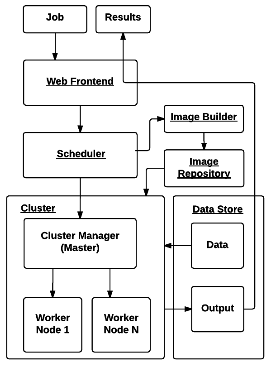
\includegraphics[scale=0.4]{img/microcloud_architecture}
\caption{Micro Cloud Architecture}
\label{fig:architecture}
\end{figure}

Cloud infrastructure consists of one or more clusters. A cluster is a collection of servers (nodes). Data storage is also part of cloud infrastructure, but is typically seperated from computing nodes and accessed over the network. Our platform consists of the following components: a web interface, a scheduler, an image builder and image repository, a cluster manager (the master node), multiple worker nodes, and a storage interface which allows reading from and writing to persistent storage. Figure \ref{fig:architecture} shows the connection between components.
\\\\
The functionality of the platform is of primary concern, thus user interface design is not considered and is outside the scope of this project. 


\subsection{System Architecture}
In Figure \ref{fig:architecture} you already saw an overview of how components interact. This section gives implementation specific details for every component.

\subsubsection{Job}
A job describes a single instance of code uploaded for execution. 
The micro cloud platform uses containers, more specifically Docker containers to execute code. Docker images are created with dockerfiles which specify the execution environment and what files to execute. Submitting a job requires a Dockerfile and source code to be executed, uploaded together packaged as a single tar archive.  

\subsubsection{Cluster Manager}
To create a cloud platform which makes use of containers, a framework is needed to manage containers in a cluster which performs scheduling and resource allocation. OpenStack was the first system considered for use as a container manager. After much trouble setting up the development environment it was decided that there are more suitable systems to solve the problem. Kubernetes has been chosen as the cluster manager framework for managing the micro cloud. 

\subsubsection{Docker Images}
A dedicated docker-in-docker container is run which is used to build docker images from dockerfiles. The image is then pushed to a private docker repository which can be accessed by any node in the cluster. The docker image is pulled by a worker node when the job is assigned to that worker node.

\subsubsection{Scheduler}
The default scheduler relies on first-in-first-out (FIFO) queues to schedule jobs. There are 3 FIFO queues: a build queue where dockerfiles are queued for the building process, a ready queue where Docker images are ready to be run, and an archiving queue where jobs are queued to have their results archived for downloading. The scheduler keeps track of running jobs using a list rather than a FIFO queue because running jobs are asynchronous. This means for example that job B can be started after job A and still still complete before job A. The number of concurrent jobs running is dependent on the number of worker nodes. Another two lists are used to keep track of completed jobs, one list for completed jobs with no results and another list for completed jobs with results ready to be downloaded. The completed jobs with no results queue is relevant because it is possible to directly interact with remote storage from within the container without using the cluster provided storage. An example of this is using object storage which isn't suited for mounting as a filesystem.

\subsubsection{Storage}
The cluster at UWC makes use of Ceph storage which can be accessed by a RADOS Block Device (RBD). Kubernetes provides support for mounting an RBD as a storage volume in a container. However due to difficulties getting Kubernetes to properly work with RBD during development, a different approach was taken. An RBD was mounted on the worker node outside of kubernetes. It was then treated as a normal filesystem and mounted as host storage in the container. Using RBD in this way is still beneficial compared to using plain host storage as raw data doesn't have to be copied to each VM, which is infeasible given the size of most raw data in Bioinformatics (The raw data used during the evaluation of the system is 36GB).

\subsubsection{Web Interface}
The backend web interface is implemented using the python flask web framework. It is a minimalist framework which allows for rapid development of web interfaces. 
The front end web interface is implemented using Angularjs to create a single page application. The website provides a form to submit a job by uploading a tar archive. Two text boxes are provided to allow the user to specify mount points (by means of an absolute file system path such as "/db" and "/results") for the raw data and results folder inside the container. Below the form is a list of jobs which shows each job's current status. This list is updated by polling the server every few seconds. If a job is complete and the results folder contains files then the user will be able to download the results as a tar archive. On a different web page (titled "regions") is a list of all available micro clouds. The user can click on a region to navigate to a different micro cloud.

\subsubsection{Community Cloud}
A community cloud is formed by implementing a centralised discovery service. This improves scalability compared to a full mesh network between micro clouds. The discovery service gives a list of connected micro clouds with their url (either an IP address or a domain) along with the name of the micro cloud. The discovery service has to be manually configured by adding a micro cloud's details to a configuration file.

\begin{figure}
\centering
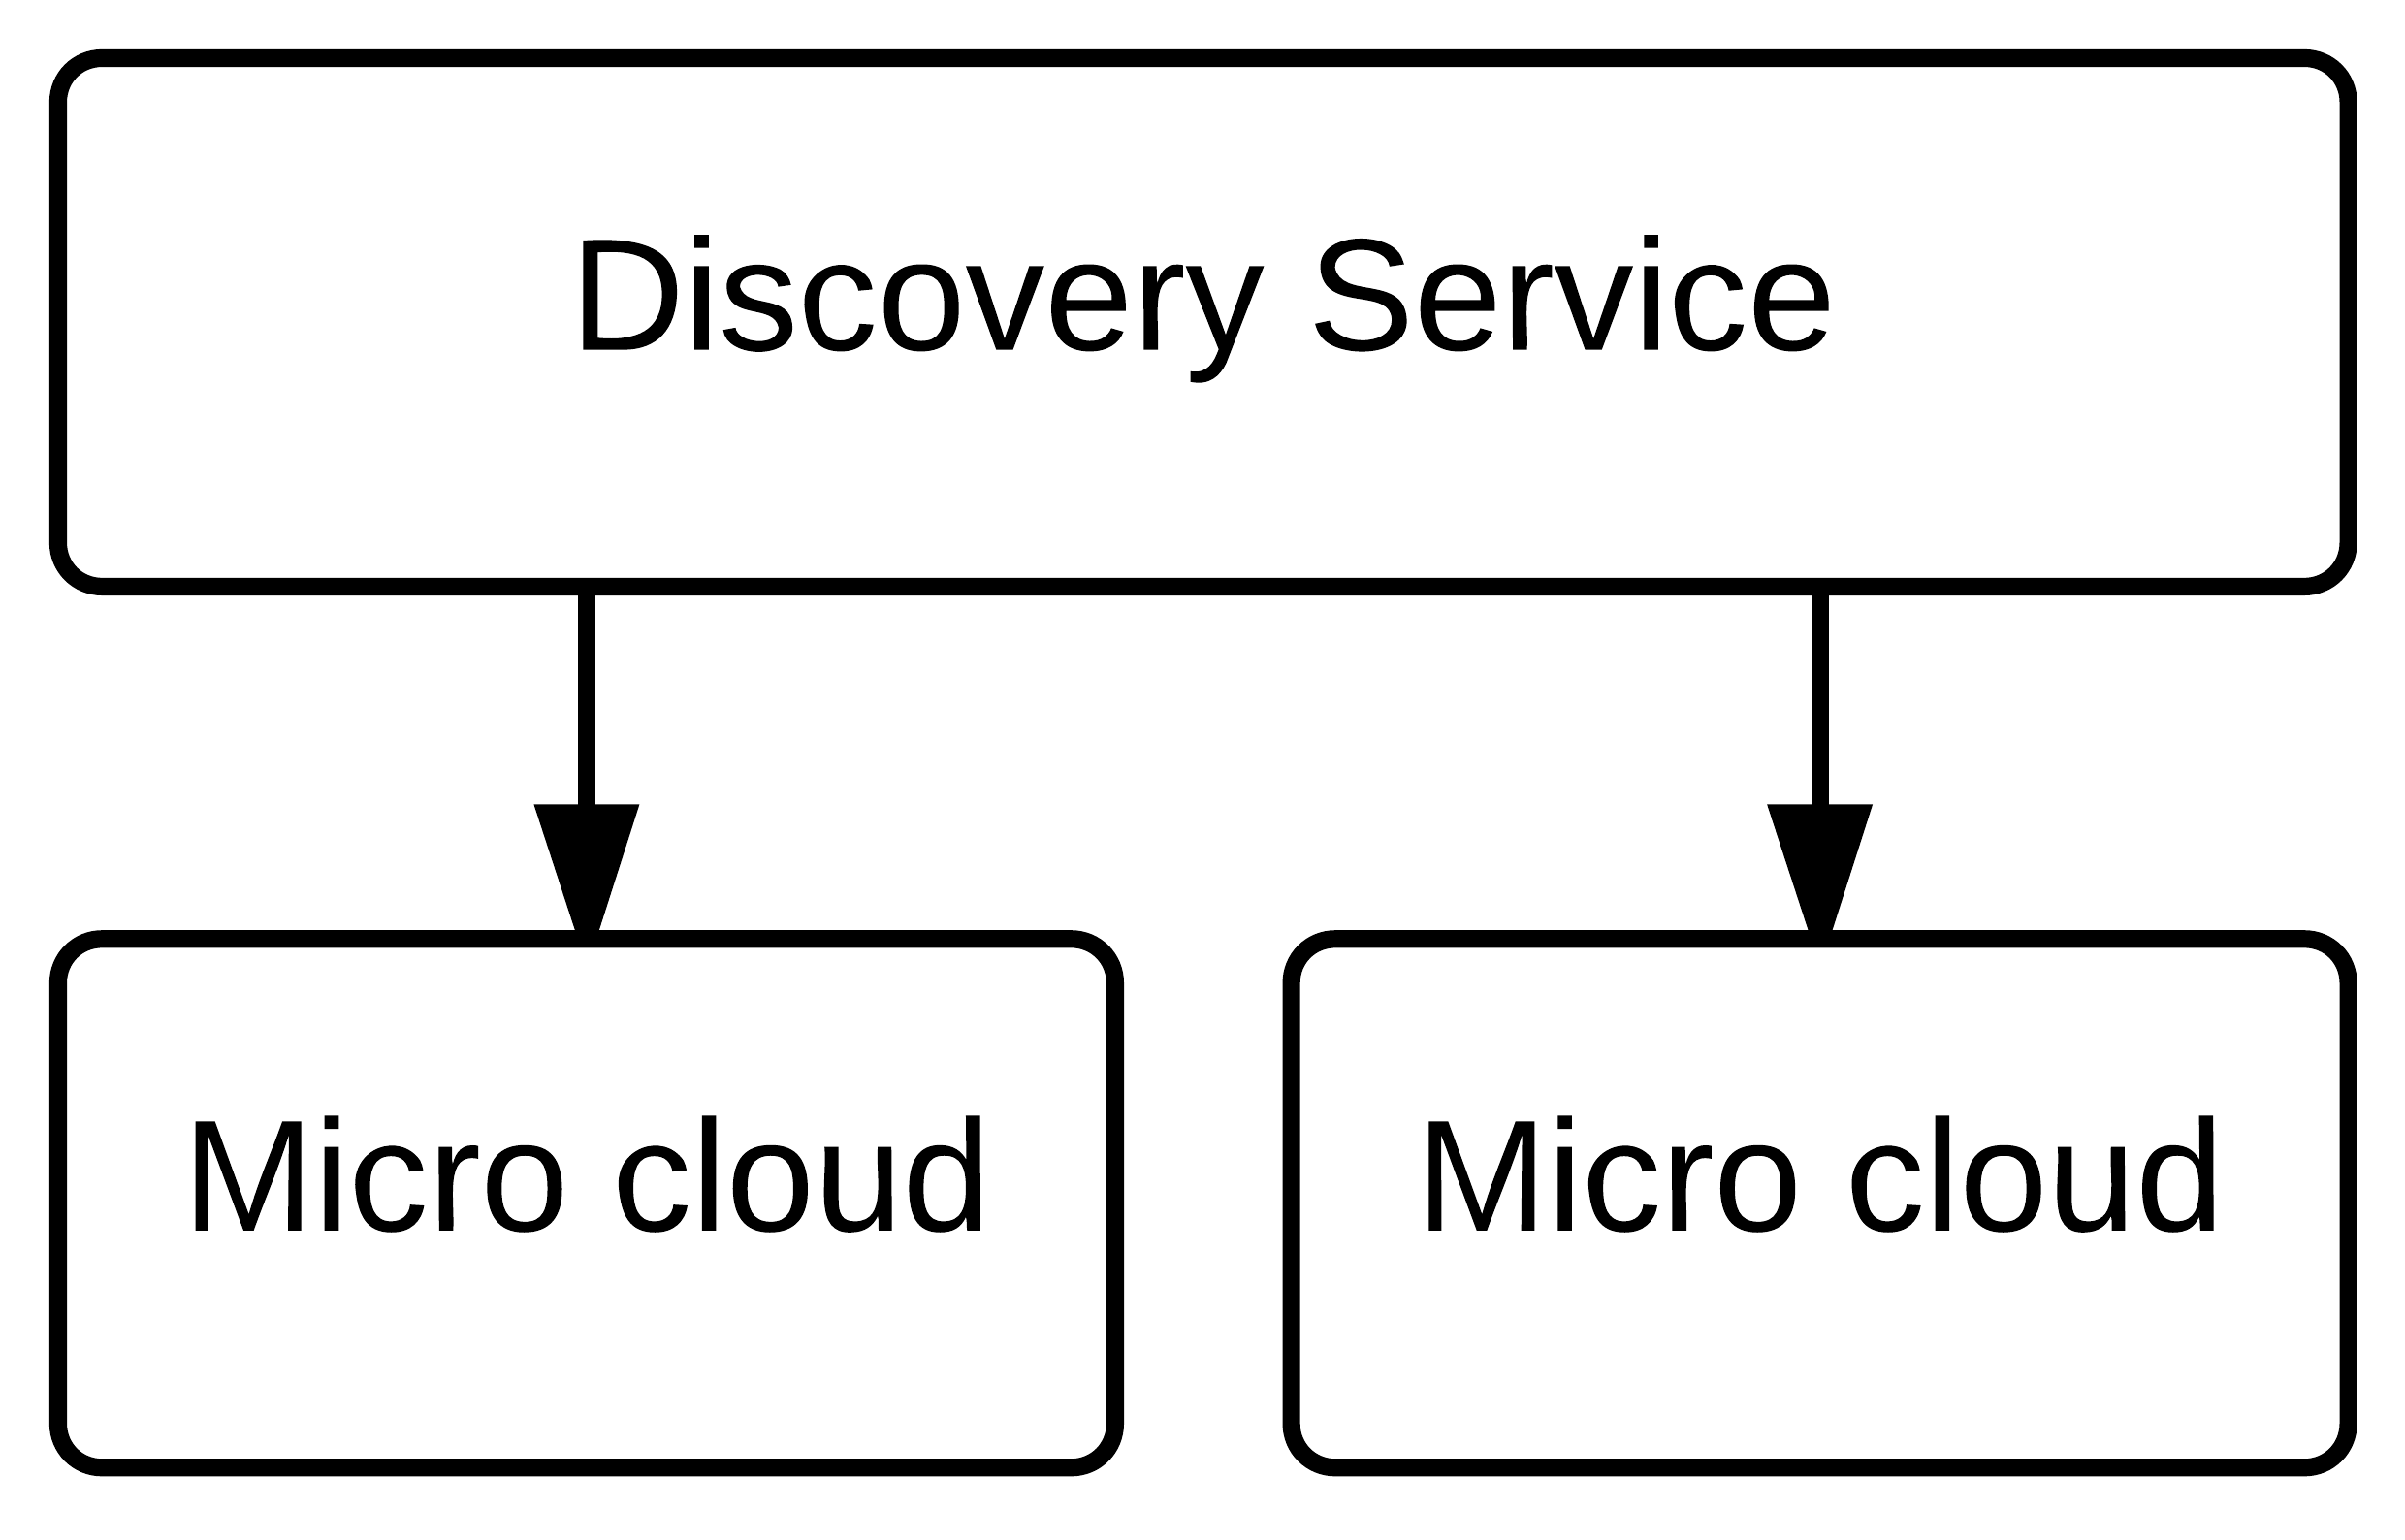
\includegraphics[scale=0.3]{img/communitycloud}
\caption{Community Cloud Architecture}
\label{fig:architecture}
\end{figure}


\subsection{Constraints}
Micro cloud deployments for evaluation are limited to UWC. The evaluation is limited to one community cloud containing two micro clouds. Each micro cloud was deployed on a single virtual machine (VM) as a single node cluster. Each VM has 1GB RAM, a single cpu, and 10GB of storage. Two 100Gb RBDs were provided, one for raw data and one for storing results. Due to both clusters residing on the same network, both clusters made use of the same storage. This wouldn't be the case if each cluster was deployed at a different institution, but for the purposes of the evaluation it isn't important.

\subsection{Software Engineering}

We implemented a proof of concept of the community cloud. The aim was not to focus on software engineering methodologies. However to allow for reproducibility the source code is stored in a Git repository hosted on Github (Git is a version control system). All the components are containerized which means a cluster can easily be deployed by running a few docker containers. This allows greater portability and reproducibility. 




\subsection{Evaluation}
The functionality of the micro cloud is evaluated by submitting sample analysis code as a job. The analysis code searches against a genome database. We chose a database that is publicly hosted by the National Center for Biotechnology Information (NCBI), an institution dedicated to improving technologies used in genomic research \cite{pruitt2005ncbi}. The analysis code makes use of the Basic Local Alignment Search Tool (BLAST) \cite{camacho2009blast}. This tool is used by specifying a database and submitting a query containing specific search criteria. Different sized jobs are tested by increasing or decreasing the size of the query, which makes it easily scalable to different sized test cases.


\section{Results and Findings}

\section{Conclusions}

\subsection{Future Work}




\bibliographystyle{ACM-Reference-Format-Journals}
\bibliography{ref} 


\end{document}
